\documentclass{ctexart}

\title{\Large 直流非平衡电桥\\{\large 实验报告}}
\author{\large  信息科学技术学院 \quad 李毅 PB22051031 \\{教室:一教1215\quad 座位号:2}}
\date{2023年10月16日}
\usepackage{amsmath}
\usepackage{amsfonts}
\usepackage{amssymb}
\usepackage{bm}
\usepackage{enumerate}
\usepackage{geometry}
\geometry{left=3.0cm,right=3.0cm,top=2.5cm,bottom=2.5cm}
\usepackage{fancyhdr}
\pagestyle{fancy}
\fancyhead[l]{ }
\fancyhead[r]{ }
\fancyhead[C]{
	\begin{tabular}{cccc}
		&\multicolumn{2}{c}\large{\textbf{中国科学技术大学物理实验报告}}\\
		\vspace{0.1cm}信息科学技术学院 & PB22051031\ 李毅 & PHYS1009B.02 & 2023年10月16日 
\end{tabular}}
\fancyfoot[C]{ 第 {\thepage} 页,共 \pageref{unknown} 页}
\renewcommand{\headrulewidth}{2pt}
\usepackage{graphicx}
\usepackage{geometry}
\usepackage[hidelinks]{hyperref}
\usepackage{multicol}
\usepackage{multirow}
\usepackage{ragged2e}
\usepackage[square,comma,numbers,super]{natbib}
\bibliographystyle{unsrt}
\usepackage{siunitx}
\usepackage{subfigure}
\usepackage{wrapfig}
\usepackage{xcolor}
\usepackage{cite}
\begin{document}
	\maketitle
    \newpage
    \section*{摘\quad 要}
    直流非平衡电桥是一种精密的测量电阻的仪器,本次实验中我们了解了其工作和组成原理,应用外接电阻箱法研究了非平衡电桥的输出的线性范围和灵敏度,并且还研究了桥臂电阻对非平衡电桥的输出的线性范围和灵敏度的影响。最后我们利用所搭建的非平衡电桥,测量铜丝的电阻温度系数。

    \section*{第一部分\quad 实验背景介绍}
    直流电桥是一种精密的电阻测量仪器,在实际工程和科学实验中具有重要的应用价值。根据测量方式,电桥可分为平衡电桥和非平衡电桥。

    平衡电桥通过将待测电阻与标准电阻进行比较,通过调节电桥使其平衡,从而得到待测电阻的值。常见的平衡电桥包括单臂直流电桥(如惠斯登电桥)和双臂直流电桥(如开尔文电桥)。然而,平衡电桥只适用于测量具有相对稳定状态的物理量。

    在实际工程和科学实验中,很多物理量是连续变化的,无法使用平衡电桥来测量。因此,需要使用非平衡电桥来测量这些物理量。非平衡电桥的基本原理是通过桥式电路来测量电阻,根据电桥输出的不平衡电压,再进行简单的线性运算处理,从而得到电阻的变化量,进而推算出引起电阻变化的其他物理量。

    \section*{第二部分\quad 实验原理和方法}
    \subsection*{2.1 \quad 实验器材}
    直流稳压电源、3个分度值为0.1$\Omega$的电阻箱,1个分度值为0.01$\Omega$的电阻箱、万用表(用作伏特表)、 Keithy2000(用作微伏表)、铜丝(漆包线)、加热台、温度计、导线等。

    \subsection*{2.2 \quad 实验原理}
    直流非平衡电桥原理如图1所示,当$\dfrac{R_3}{R_2}=\dfrac{R_4}{R_1}$时,电桥平衡。$U_g=0$。当用$R_4+ \Delta R$代替$R_4$时,$\dfrac{R_3}{R_2} \neq \dfrac{R_4+ \Delta R}{R_1}$,此时$U_g \neq 0$,为非平衡状态。

    ~\\
    \begin{minipage}[c]{1\textwidth}
        \centering 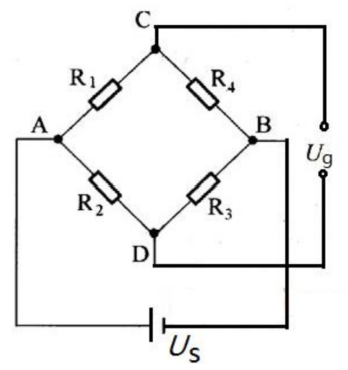
\includegraphics[scale=1]{1} \\\small{图2.1 非平衡电桥电路图}
    \end{minipage}
    ~\\

    $U_g$使用理想高精度电压表测出。用电路分析有关知识,输出的非平衡电压为:

    $$ U_g=\dfrac{R_2 R_4+R_2 \Delta R-R_1 R_3}{(R_1+R_4)(R_2+R_3)+\Delta R(R_2+R_3)}U_s \quad (1)$$

    本实验中,为简化计算,使用等臂电桥,代入等臂条件:$R_1=R_2=R_3=R_4=R_0$,并称电阻的应变量为$\delta=\dfrac{\Delta R}{R_0}$。将其代入(1)式,得到:
    $$U_g=\dfrac{U_s}{4} \delta \dfrac{1}{1+\frac{1}{2}\delta}\quad (2)$$

    若$\Delta R \ll R_0$,即$\delta \rightarrow 0$时,有:
    $$U_g=\dfrac{U_s}{4}\delta=\dfrac{U_s}{4 R_0}\Delta R \quad (3)$$
    这样, 非平衡电桥输出电压$U_g$与桥臂电阻的变化量$\Delta R$成正比,为线性关系。 

    若$\Delta R$较大,(2)式中的$\dfrac{\delta}{2}$项不能省略,此时$U_g$与$\delta$呈非线性关系。

    \section*{第三部分\quad 实验内容和步骤}
\subsection*{3.1 \quad 实验一:研究非平衡电桥的输出的线性范围和灵敏度}
用外接电阻箱法研究非平衡电桥的$U_g$与$\delta$关系,作出$U_g - \delta$曲线,并对此实验曲线与理想直线(式(3)) 之间进行误差分析, 以确定电桥输出的线性范围和灵敏度。

实验步骤如下:
\begin{enumerate}[(1)]
    \item 调节电源输出电压,同时用万用表直流电压档来校准,使其输出电压为$U_s$ = 2.0V。电路如图 1 所示并用导线连接好,用高精度台式万用表(Keithy2000)来测量$U_g$。
    \item 先取电桥为等臂,即: $R_1=R_2=R_3=R_4=R_0=1k\Omega$,由于导线存在有一定的电阻,微调$R_3$的值,使$U_g$为零,此时电桥平衡,并记录$R_3$的具体值。
    \item 改变$R_4$从 800 至 1200 $\Omega$,每次变化量为 20 $\Omega$, 按顺序记下各$U_g$的值,作出$U_g - \delta$曲线。
    \item 根据公式(3) 过原点作一条直线 $U_g^{\text{理论}} - \delta$, 并与实际测量的$U_g^{\text{实测}} - \delta$曲线进行比较, 得出$U_g - \delta$的线性关系成立的$\delta$取值范围。
    \item 测算在此桥臂电阻值下,电桥在零点附近的绝对灵敏度。
\end{enumerate}

\subsection*{3.2 \quad 实验二:研究桥臂电阻对非平衡电桥的输出的线性范围和灵敏度的影响}
保持电源电压$U_s=2.0V$不变,改变$R_0$的值,研究非平衡电桥的线性范围和灵敏度与$R_0$的关系。

实验步骤如下:
\begin{enumerate}[(1)]
    \item 电路图仍如图 1 所示,保持电源电压$U_s=2.0V$不变,取电桥为等臂,即$R_1=R_2=R_3=R_4=R_0$,$R_0$改取5000$\Omega$和$50\Omega$,微调$R_3$的值,使$U_g$为零,此时电桥平衡,并记录$R_3$的具体值。
    \item 改变$R_4$的阻值,每次改变量为$\dfrac{R_4}{2\%}$。 取值范围取$(R_0 −20\%R_0, R_0 + 20\%R_0)$。 记录桥路输出电压数据,画图测算线性范围,并计算电桥在零点附近的绝对灵敏度。
    \item 结合实验一数据,分析$U_g$与$\delta$之间近似 满足线性关系时的$R_4$取值范围,此范围的长度$\Delta R_4$与$R_0$大小之间的关系;同时分析实测零点绝对灵敏度大小 与$R_0$大小之间的关系。
\end{enumerate}

\subsection*{3.3 \quad 实验三:使用非平衡电桥测量铜丝的电阻温度系数}
利用搭建的直流非平衡电桥, 测量并记录铜丝的电阻,以及其电阻随温度的改变值。 计算铜丝的电阻温度系数, 在 0$^\circ C$和 20$^\circ C$时的值和不确定度。

实验步骤如下:
\begin{enumerate}[(1)]
    \item 由于铜丝电阻较小,取桥臂电阻为 50$\Omega$,用 Keithy2000来测量桥路输出电压$U_g$。 保持恒压源输出电压为 2.0V, 微调$R_3$的值,使$U_g$尽可能的小($<\left\lvert 0.01 mV \right\rvert $),并记录对应的$U_\text{g0min}$。
    \item 把 3m 长,直径为 0.60mm 的 铜丝(漆包线)串联到$R_4$所在的桥臂上。把铜丝浸没在陶瓷杯内的水中,用温度计测量水温 t, 记录水温并测量当前水温下桥路输出电压$U_g(t)$值,并与没有串联 铜 丝时$U_{g0min}$比较。
    \item 用加热台对杯子里水进行加热, 铜丝温度缓慢上升。 每隔 5$^\circ C$记录一下对应的$U_g(t)$,直到 85$^\circ C$ 为止。
    \item 根据各个不同温度点下的$U_g(t)$值(与没有串联 铜丝时$U_\text{g0min}$比较),利用简单的线性关系(式(3)), 计算出铜丝在各个温度点下的电阻值$R_{Cu(t)}$,并作出$R_{Cu(t)}-t$的散点图以及拟合直线。 求出拟合直线的斜率,并推算 0$^\circ C$和 20$^\circ C$时的铜丝电阻。
    \item  根据电阻温度系数定义式$\alpha_T=k/R_T$, 计算 铜 丝的在0$^\circ C$和 20$^\circ C$处的电阻温度系数$\alpha_t$, 以及在 $P = 95\%$置信概率下的相对不确定度$u_\alpha/\alpha$和绝对不确定度$u_\alpha$(A 类不确定度)。
   
\end{enumerate}
    \section*{第四部分\quad 实验数据和分析}
    \subsection*{4.1 \quad 实验一:研究非平衡电桥的输出的线性范围和灵敏度}
    \subsubsection*{4.1.1 实验数据}
\begin{table}[!ht]
    \centering 表1:$R_0$ = 1$k\Omega$时, 桥路二端点 C、 D 输出电压差与桥臂电阻改变量$\Delta R$的关系($R_3=1000.06\Omega$)
    \resizebox*{\textwidth}{!}{
        \begin{tabular}{|c|c|c|c|c|c|c|c|c|c|c|c|}
            \hline
            $R_4/\Omega$              & 800      & 820     & 840     & 860     & 880     & 900     & 920     & 940     & 960     & 980     & 1000   \\ \hline
            $\Delta R=R_4-R_0/\Omega$ & -200     & -180    & -160    & -140    & -120    & -100    & -80     & -60     & -40     & -20     & 0      \\ \hline
            $\delta=\Delta R/R_0$       & -20\%    & -18\%   & -16\%   & -14\%   & -12\%   & -10\%   & -8\%    & -6\%    & -4\%    & -2\%    & 0\%    \\ \hline
            $U_g(mV)$                 & -111.249 & -99.034 & -87.082 & -75.389 & -63.944 & -52.742 & -41.772 & -31.027 & -20.502 & -10.189 & -0.005 \\ \hline\hline
            $R_4/\Omega$              & 1020     & 1040    & 1060    & 1080    & 1100    & 1120    & 1140    & 1160    & 1180    & 1200    &        \\ \hline
            $\Delta R=R_4-R_0/\Omega$ & 20       & 40      & 60      & 80      & 100     & 120     & 140     & 160     & 180     & 200     &        \\ \hline
            $\delta=\Delta R/R_0$       & 2\%      & 4\%     & 6\%     & 8\%     & 10\%    & 12\%    & 14\%    & 16\%    & 18\%    & 20\%    &        \\ \hline
            $U_g(mV)$                 & 9.906    & 19.615  & 29.136  & 38.475  & 47.631  & 56.619  & 65.439  & 74.095  & 82.593  & 90.932  &        \\ \hline
            \end{tabular}
    }
\end{table}
\subsubsection*{4.1.2 测算线性关系成立范围}
    根据此表做出$U_g-\delta$拟合曲线。根据公式(3)过原点做一条直线$U_g^{\text{理论}}=500\delta$,令$U_\delta=\dfrac{\left\lvert U_g^{\text{实测}}-U_g^{\text{理论}}\right\rvert }{\left\lvert U_g^{\text{理论}}\right\rvert }$,并做出$U_\delta-\delta$关系图,当$U_\delta<0.05$时,即认为$U_g - \delta$线性关系成立。
    
    ~\\
    \begin{minipage}[c]{0.5\textwidth}
        \centering 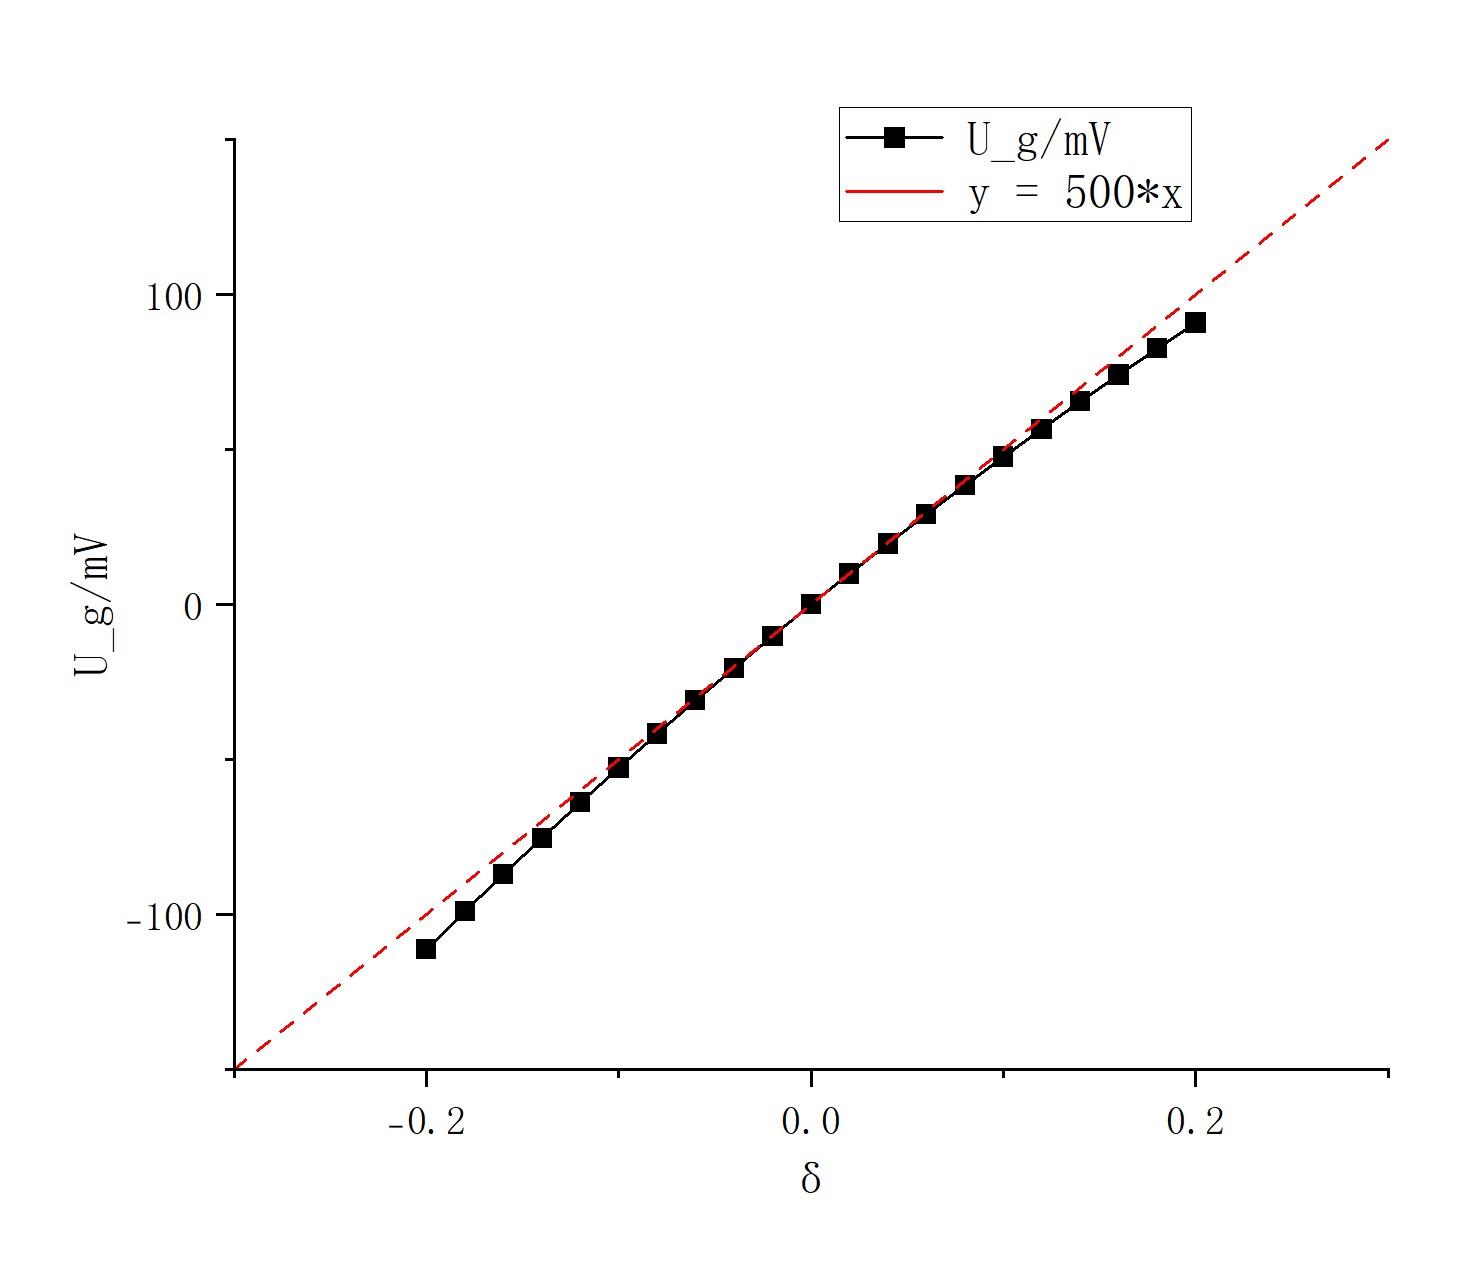
\includegraphics[scale=0.4]{1.1.1} \\\small{图4.1.1 $R_0=1000\Omega$时$U_g^{\text{理论}} - \delta$直线以及$U_g^{\text{实际}} - \delta$拟合曲线}
    \end{minipage}
    \begin{minipage}[c]{0.5\textwidth}
        \centering 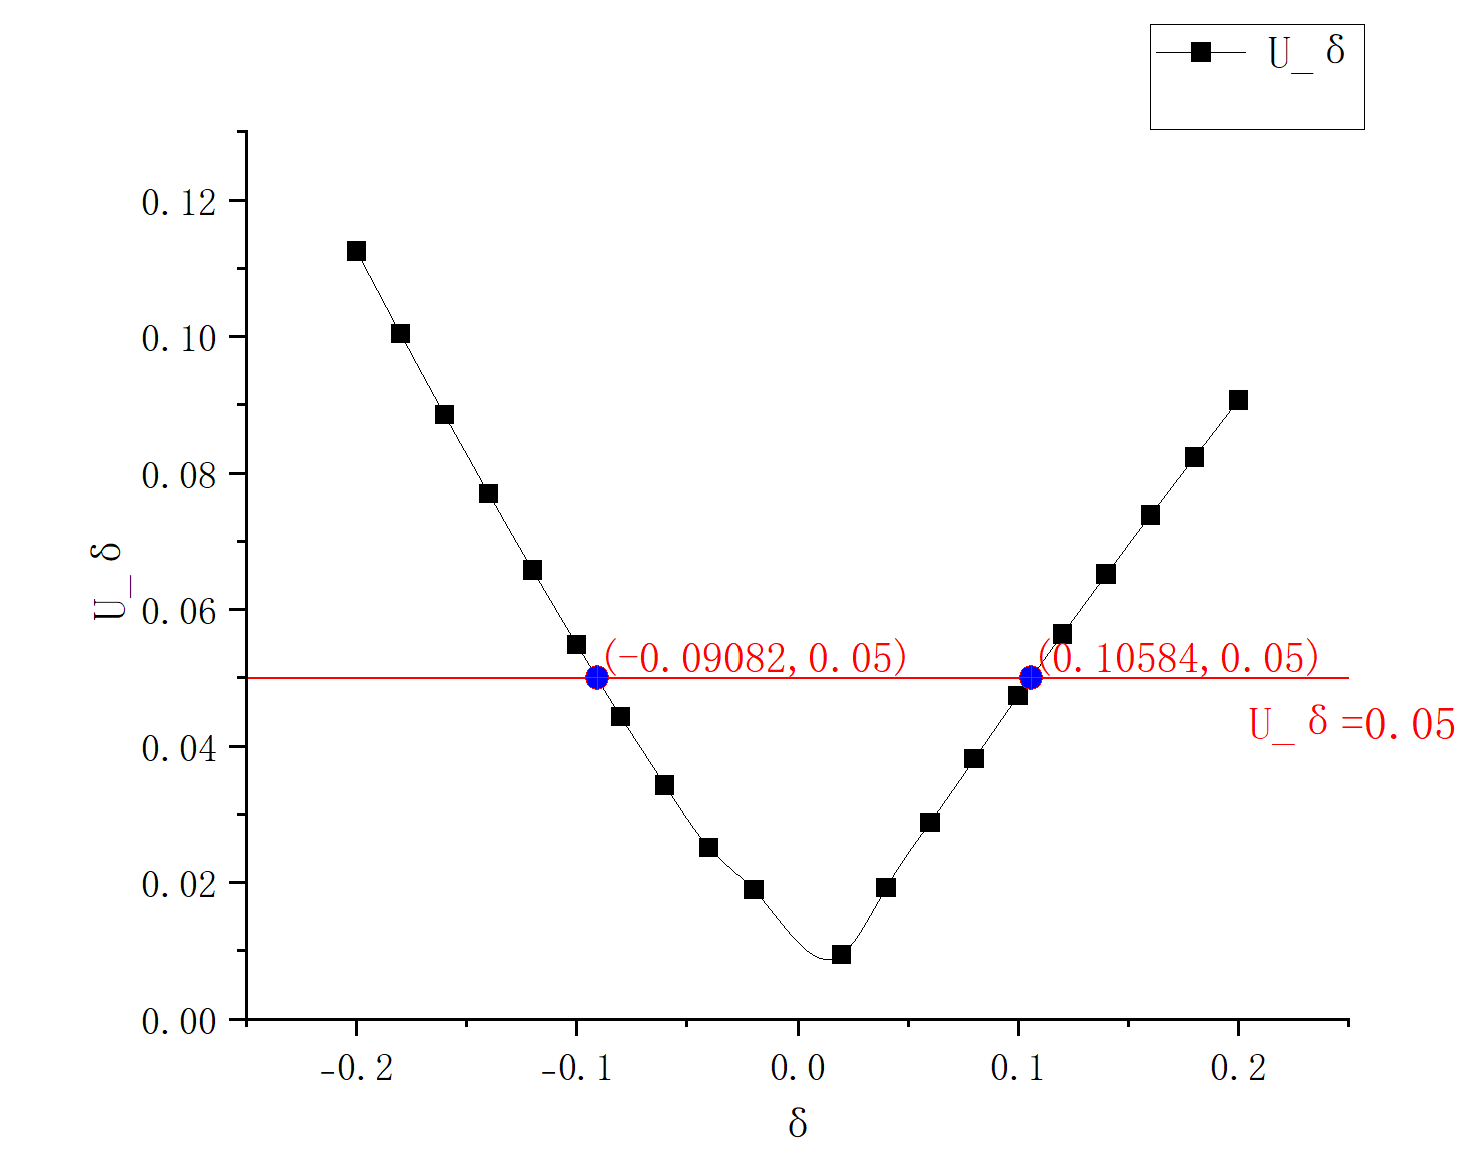
\includegraphics[scale=0.4]{1.1.2} \\\small{图4.1.2 $R_0=1000\Omega$时$U_\delta -\delta $关系图}
    \end{minipage}
    ~\\

    如图4.1.1,图4.1.2所示,$U_g - \delta$线性关系成立的$\delta$取值范围为$-0.09082<\delta<0.10584$,与理论值:$-0.09524<\delta<0.10526$左误差为4.64\%,右端点误差为0.55\%,均小于5\%,误差在合理范围内。此时$R_4$取值范围为$909.18\Omega<R_4<1105.84\Omega$。
    \subsubsection*{4.1.3 测算电桥在零点附近的绝对灵敏度}

    绝对灵敏度的公式为$S=\lim_{\Delta R \to 0}\dfrac{\Delta U_g}{\Delta R} =\dfrac{1}{R_0} \lim_{\Delta \delta \to 0}\dfrac{\Delta U_g}{\Delta \delta} $,因此,可以对4.1.1中的拟合曲线进行求导,得到$\lim_{\Delta \delta \to 0}\dfrac{\Delta U_g}{\Delta \delta} -\delta$关系,如图4.1.3所示的曲线所示。再除以$R_0$值即可得到绝对灵敏度S。
    
    ~\\
    \begin{minipage}[c]{1\textwidth}
        \centering 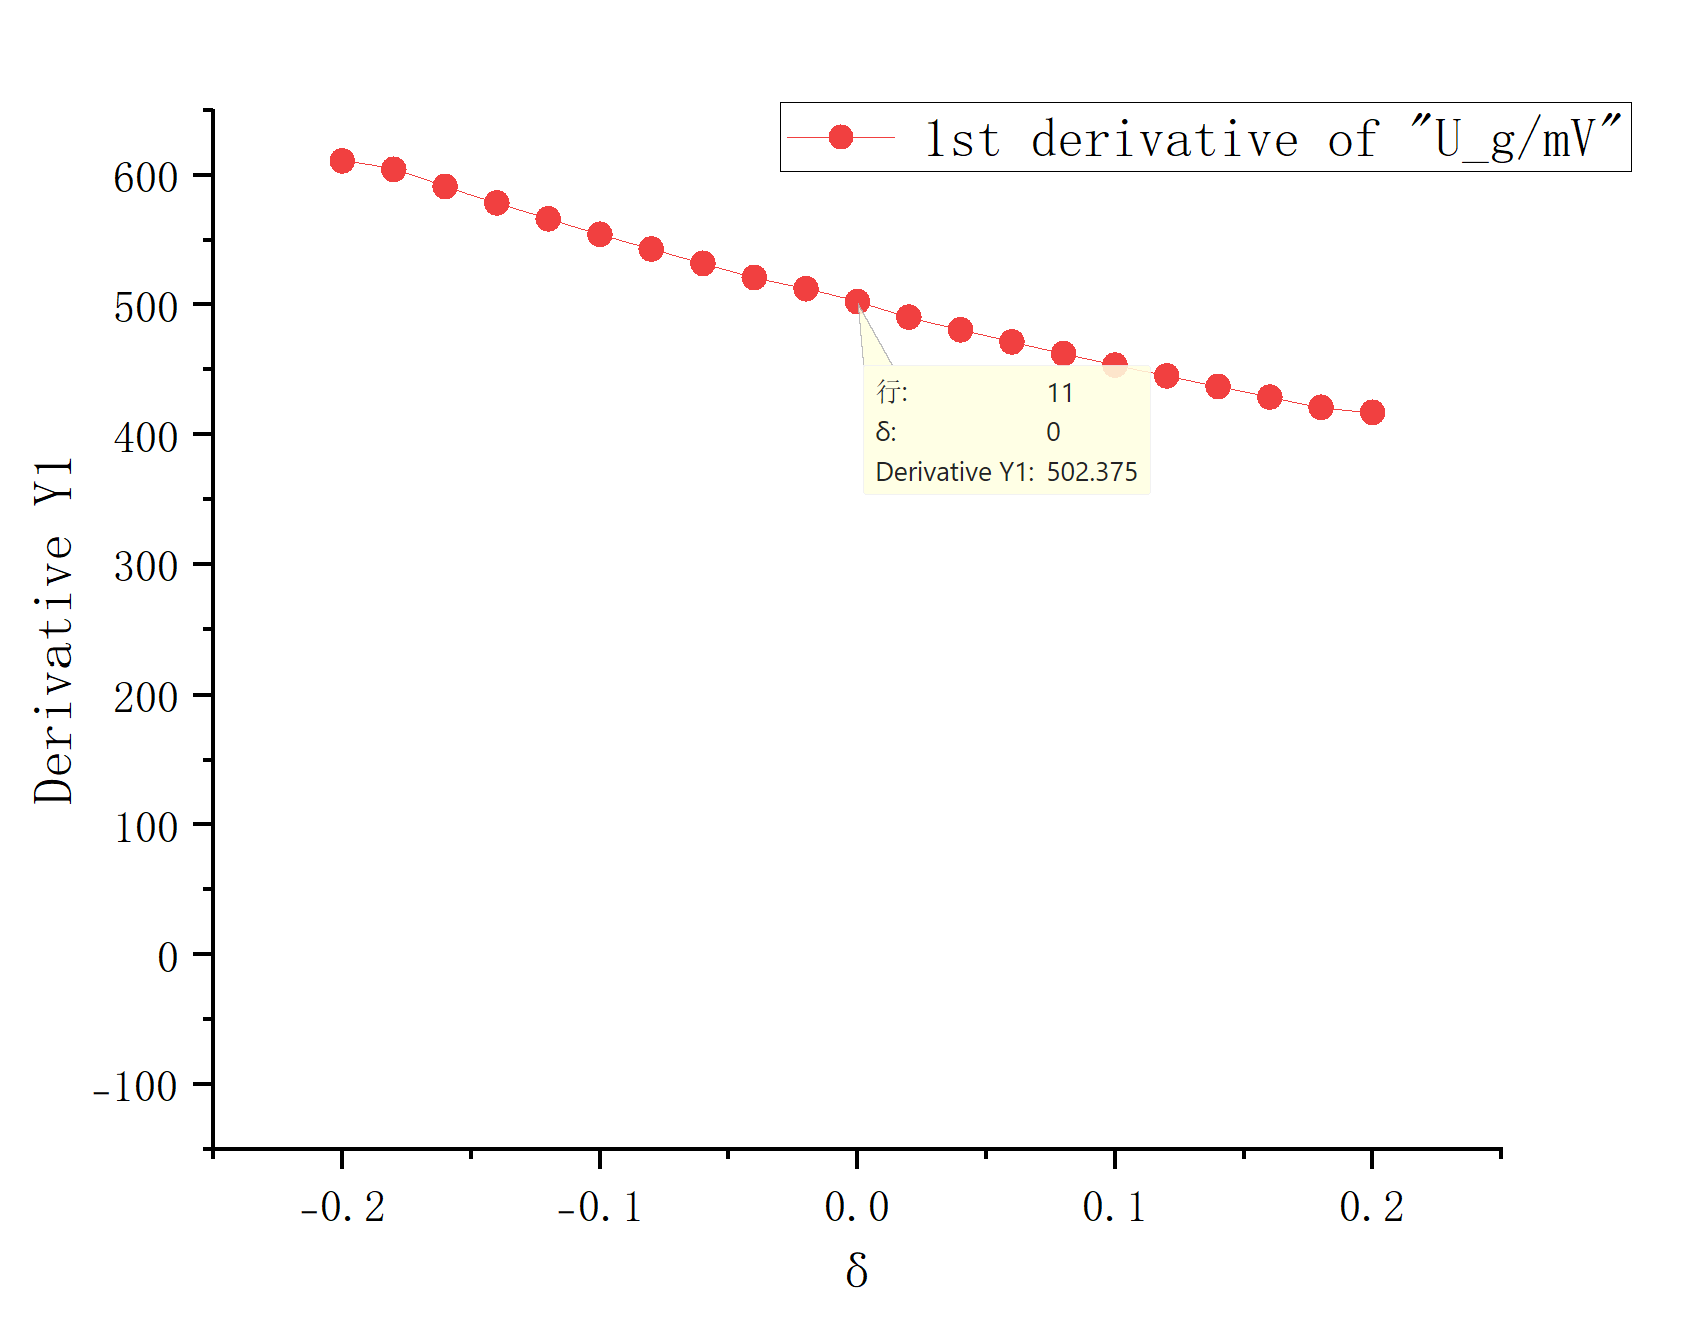
\includegraphics[scale=0.4]{1.1.3} \\\small{图4.1.3 $R_0=1000\Omega$时$U_g^{\text{实际}} - \delta$拟合曲线的导数曲线}
    \end{minipage}
    ~\\

    如图4.1.3所示,在$\delta=0$处,绝对灵敏度为0.502375$mV/\Omega$

    \subsection*{4.2 \quad 实验二:研究桥臂电阻对非平衡电桥的输出的线性范围和灵敏度的影响}

    \subsubsection*{4.2.1 当$R_0$=5000$\Omega$时}
    实验数据如下表
    \begin{table}[!ht]
        \centering  表2:$R_0$ = 5$k\Omega$时, 桥路二端点 C、 D 输出电压差与桥臂电阻改变量$\Delta R$的关系($R_3=5000.34\Omega$)
        \resizebox*{\textwidth}{!}{
        \begin{tabular}{|c|c|c|c|c|c|c|c|c|c|c|c|}
        \hline
        $R_4/\Omega$              & 4000     & 4100    & 4200    & 4300    & 4400    & 4500    & 4600    & 4700    & 4800    & 4900    & 5000  \\ \hline
        $\Delta R=R_4-R_0/\Omega$ & -1000    & -900    & -800    & -700    & -600    & -500    & -400    & -300    & -200    & -100    & 0     \\ \hline
        $\delta=\Delta R/R_0$       & -20\%    & -18\%   & -16\%   & -14\%   & -12\%   & -10\%   & -8\%    & -6\%    & -4\%    & -2\%    & 0\%   \\ \hline
        $U_g(mV)$                 & -111.181 & -98.966 & -87.018 & -75.323 & -63.877 & -52.674 & -41.701 & -30.978 & -20.433 & -10.122 & 0.001 \\ \hline\hline
        $R_4/\Omega$              & 5100     & 5200    & 5300    & 5400    & 5500    & 5600    & 5700    & 5800    & 5900    & 6000    &       \\ \hline
        $\Delta R=R_4-R_0/\Omega$ & 100      & 200     & 300     & 400     & 500     & 600     & 700     & 800     & 900     & 1000    &       \\ \hline
        $\delta=\Delta R/R_0$       & 2\%      & 4\%     & 6\%     & 8\%     & 10\%    & 12\%    & 14\%    & 16\%    & 18\%    & 20\%    &       \\ \hline
        $U_g(mV)$                 & 9.905    & 19.615  & 29.138  & 38.480  & 47.642  & 56.632  & 65.453  & 74.111  & 82.609  & 90.973  &       \\ \hline
        \end{tabular}
        }
        \end{table}

    同实验一,根据此表做出$U_g-\delta$拟合曲线。根据公式(3)过原点做一条直线$U_g^{\text{理论}}=500\delta$,令$U_\delta=\dfrac{\left\lvert U_g^{\text{实测}}-U_g^{\text{理论}}\right\rvert }{\left\lvert U_g^{\text{理论}}\right\rvert }$,并做出$U_\delta-\delta$关系图。

    ~\\
    \begin{minipage}[c]{0.5\textwidth}
        \centering 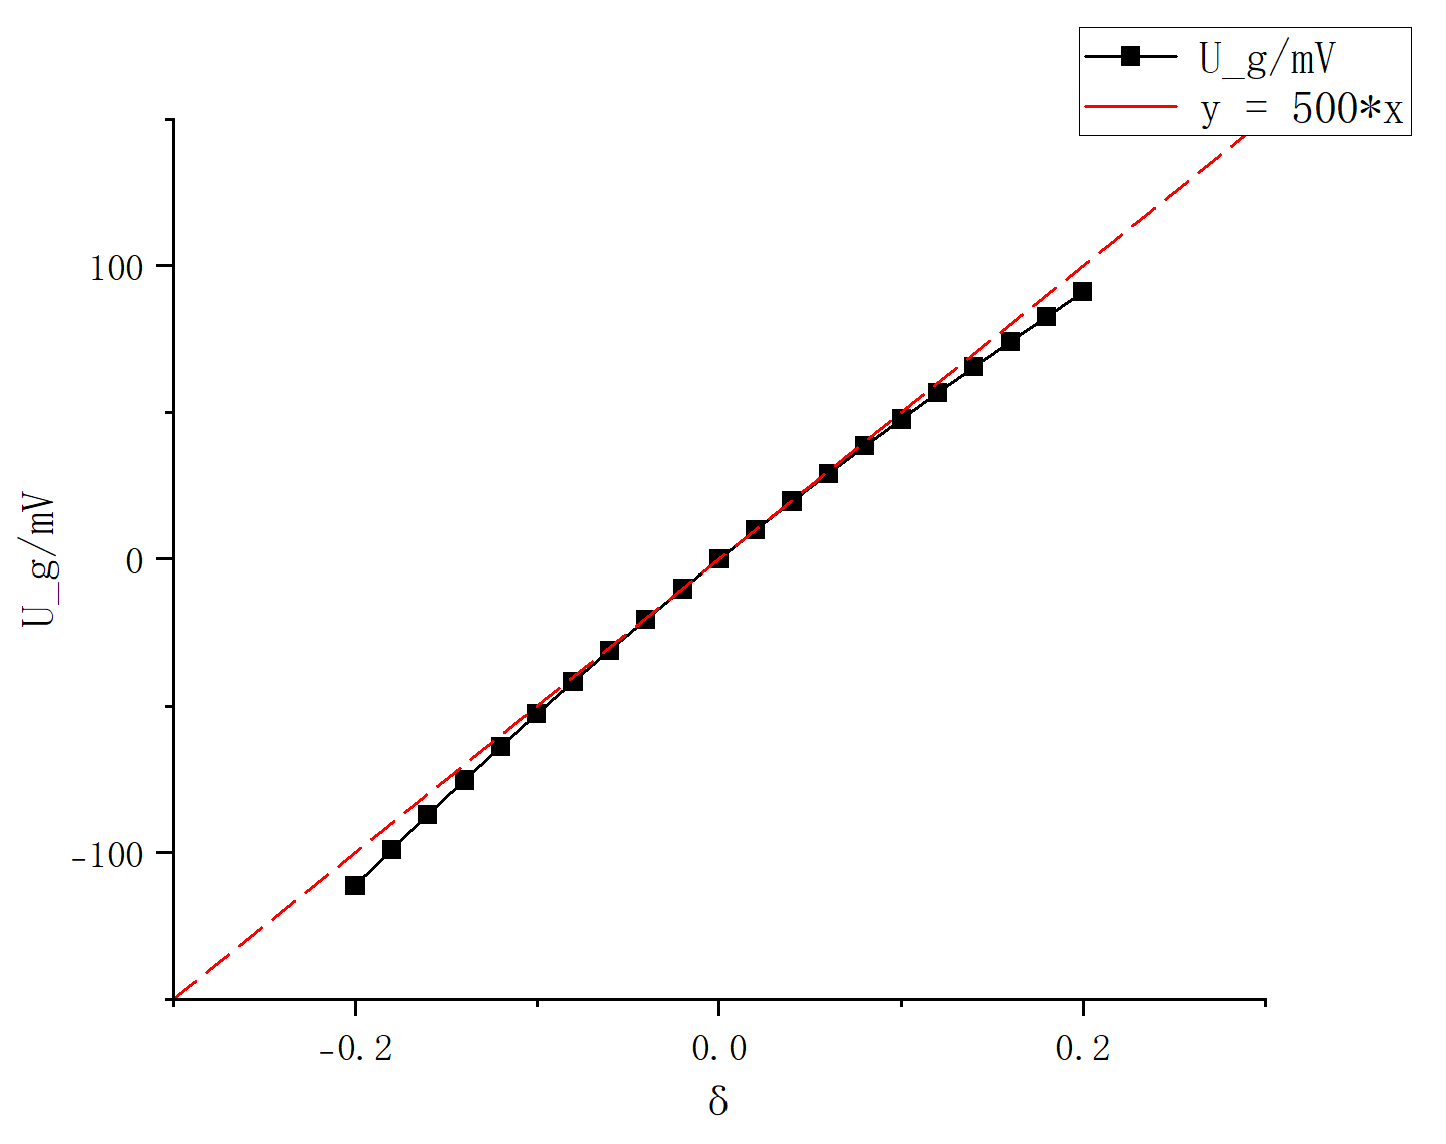
\includegraphics[scale=0.4]{2.1.1} \\\small{图4.2.1 $R_0=5000\Omega$时$U_g^{\text{理论}} - \delta$直线以及$U_g^{\text{实际}} - \delta$拟合曲线}
    \end{minipage}
    \begin{minipage}[c]{0.5\textwidth}
        \centering 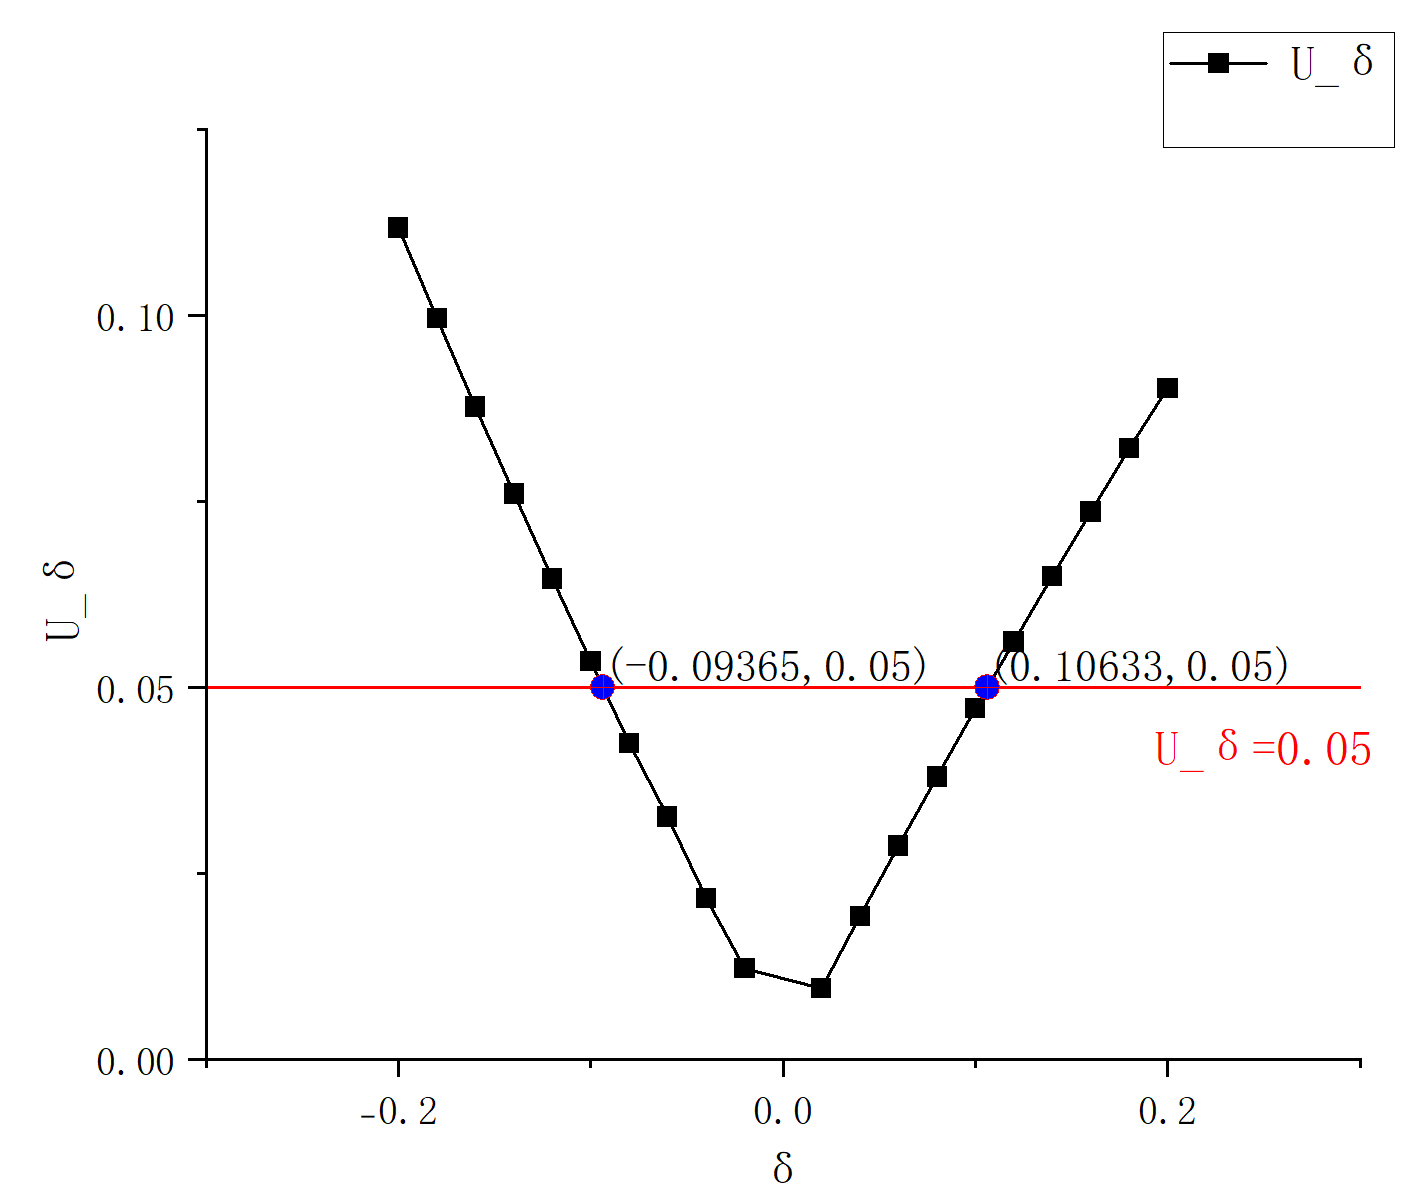
\includegraphics[scale=0.4]{2.1.2} \\\small{图4.2.2 $R_0=5000\Omega$时$U_\delta -\delta $关系图}
    \end{minipage}
    ~\\

    如图4.2.1,图4.2.2所示,$U_g - \delta$线性关系成立的$\delta$取值范围为$-0.09365<\delta<0.10633$,与理论值:$-0.09524<\delta<0.10526$左误差为1.67\%,右端点误差为1.02\%,均小于5\%,误差在合理范围内。此时$R_4$取值范围为$4531.75\Omega<R_4<5531.65\Omega$。

    ~\\
    \begin{minipage}[c]{1\textwidth}
        \centering 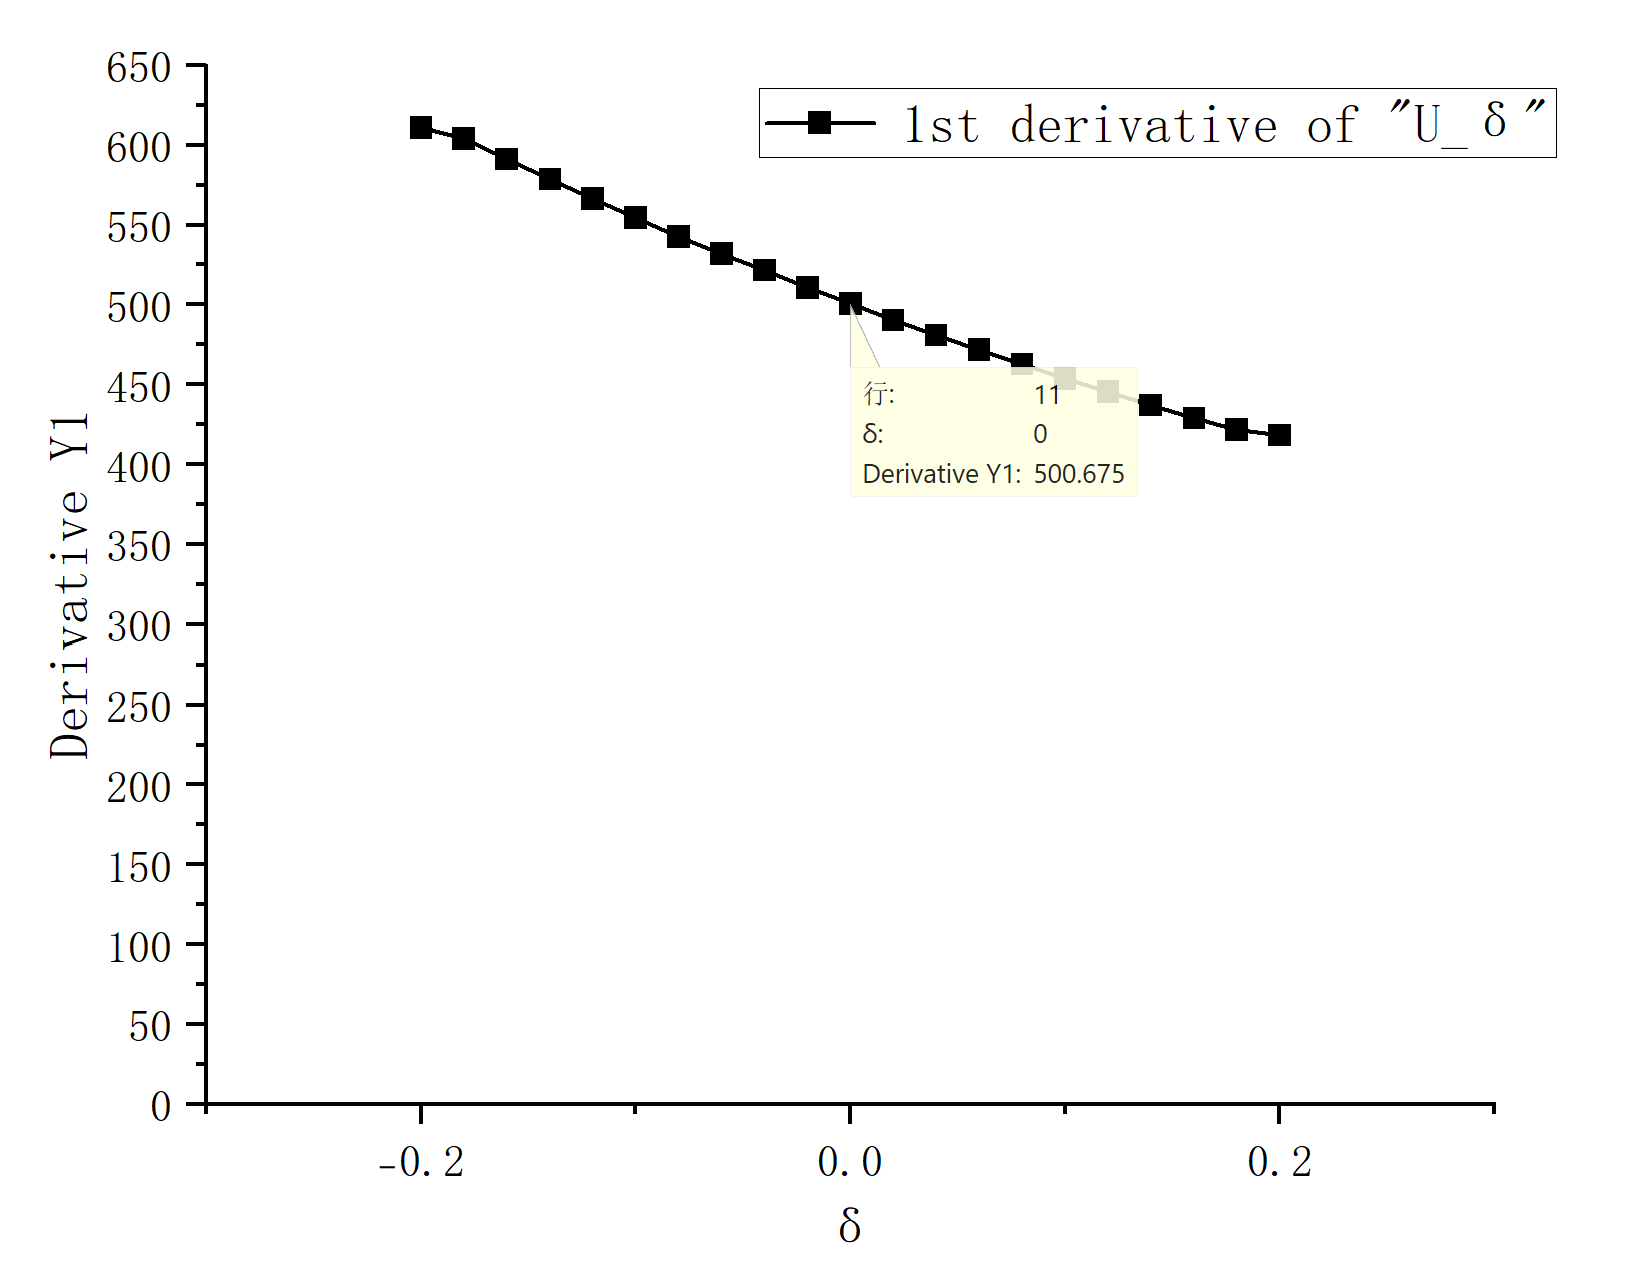
\includegraphics[scale=0.4]{2.1.3} \\\small{图4.2.3 $R_0=5000\Omega$时$U_g^{\text{实际}} - \delta$拟合曲线的导数曲线}
    \end{minipage}
    ~\\

    同实验一方法,如图4.2.3所示,在$\delta=0$处,绝对灵敏度为0.100135$mV/\Omega$

    \subsubsection*{4.2.2 当$R_0$=50$\Omega$时}
    实验数据如下表
    \begin{table}[!ht]
        \centering  表3:$R_0$ = 50$\Omega$时, 桥路二端点 C、 D 输出电压差与桥臂电阻改变量$\Delta R$的关系($R_3=50.01\Omega$)
        \resizebox*{\textwidth}{!}{
            \begin{tabular}{|c|c|c|c|c|c|c|c|c|c|c|c|}
                \hline
                $R_4/\Omega$              & 40       & 41      & 42      & 43     & 44      & 45      & 46      & 47      & 48      & 49      & 50     \\ \hline
                $\Delta R=R_4-R_0/\Omega$ & -10      & -9      & -8      & -7     & -6      & -5      & -4      & -3      & -2      & -1      & 0      \\ \hline
                $\delta=\Delta/R_0$       & -20\%    & -18\%   & -16\%   & -14\%  & -12\%   & -10\%   & -8\%    & -6\%    & -4\%    & -2\%    & 0\%    \\ \hline
                $U_g(mV)$                 & -110.909 & -98.773 & -86.802 & -75.17 & -63.679 & -52.562 & -41.574 & -30.884 & -20.352 & -10.083 & -0.025 \\ \hline
                $R_4/\Omega$              & 51       & 52      & 53      & 54     & 55      & 56      & 57      & 58      & 59      & 60      &        \\ \hline
                $\Delta R=R_4-R_0/\Omega$ & 1        & 2       & 3       & 4      & 5       & 6       & 7       & 8       & 9       & 10      &        \\ \hline
                $\delta=\Delta/R_0$       & 2\%      & 4\%     & 6\%     & 8\%    & 10\%    & 12\%    & 14\%    & 16\%    & 18\%    & 20\%    &        \\ \hline
                $U_g(mV)$                 & 9.854    & 19.583  & 29.063  & 38.422 & 47.539  & 56.536  & 65.32   & 74.008  & 82.451  & 90.799  &        \\ \hline
                \end{tabular}
        }
        \end{table}

    同实验一,根据此表做出$U_g-\delta$拟合曲线。根据公式(3)过原点做一条直线$U_g^{\text{理论}}=500\delta$,令$U_\delta=\dfrac{\left\lvert U_g^{\text{实测}}-U_g^{\text{理论}}\right\rvert }{\left\lvert U_g^{\text{理论}}\right\rvert }$,并做出$U_\delta-\delta$关系图。

    ~\\
    \begin{minipage}[c]{0.5\textwidth}
        \centering 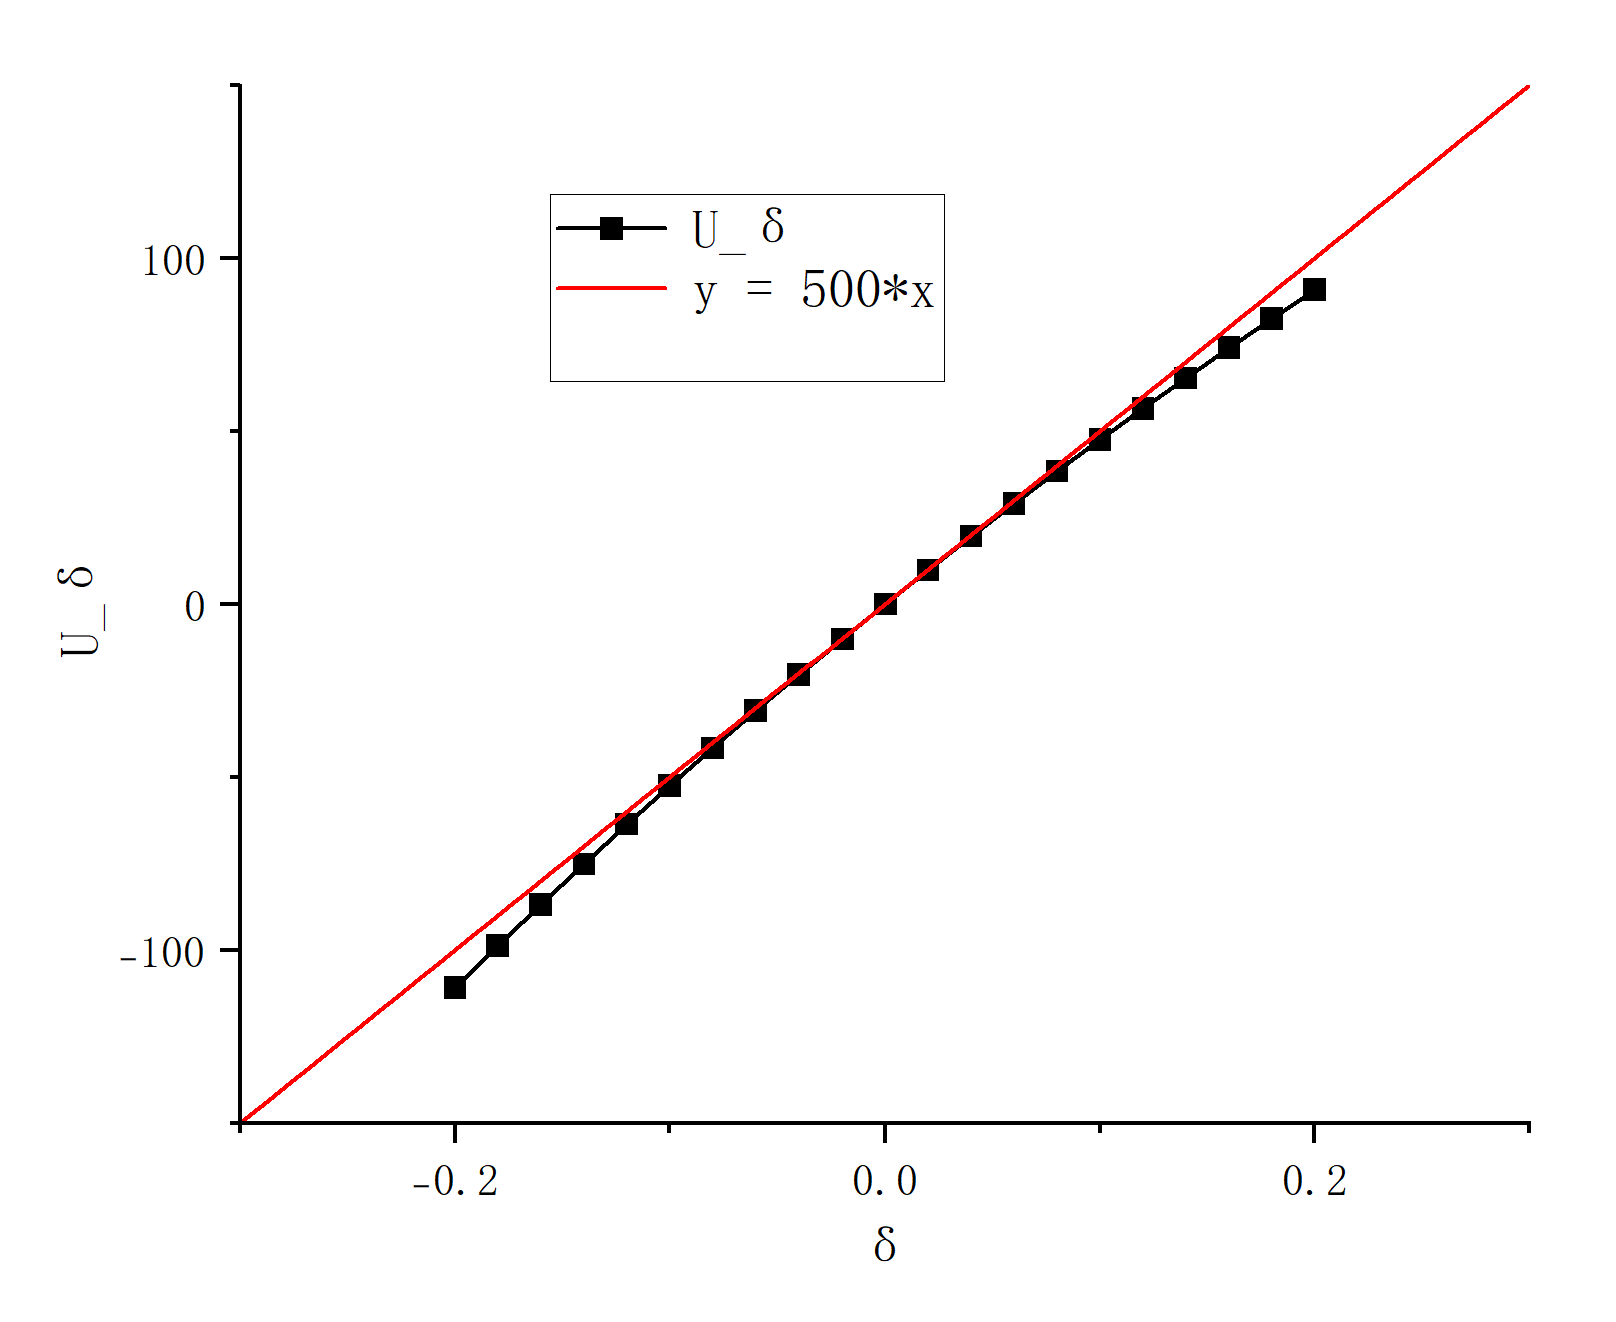
\includegraphics[scale=0.4]{3.1.1} \\\small{图4.3.1 $R_0=50\Omega$时$U_g^{\text{理论}} - \delta$直线以及$U_g^{\text{实际}} - \delta$拟合曲线}
    \end{minipage}
    \begin{minipage}[c]{0.5\textwidth}
        \centering 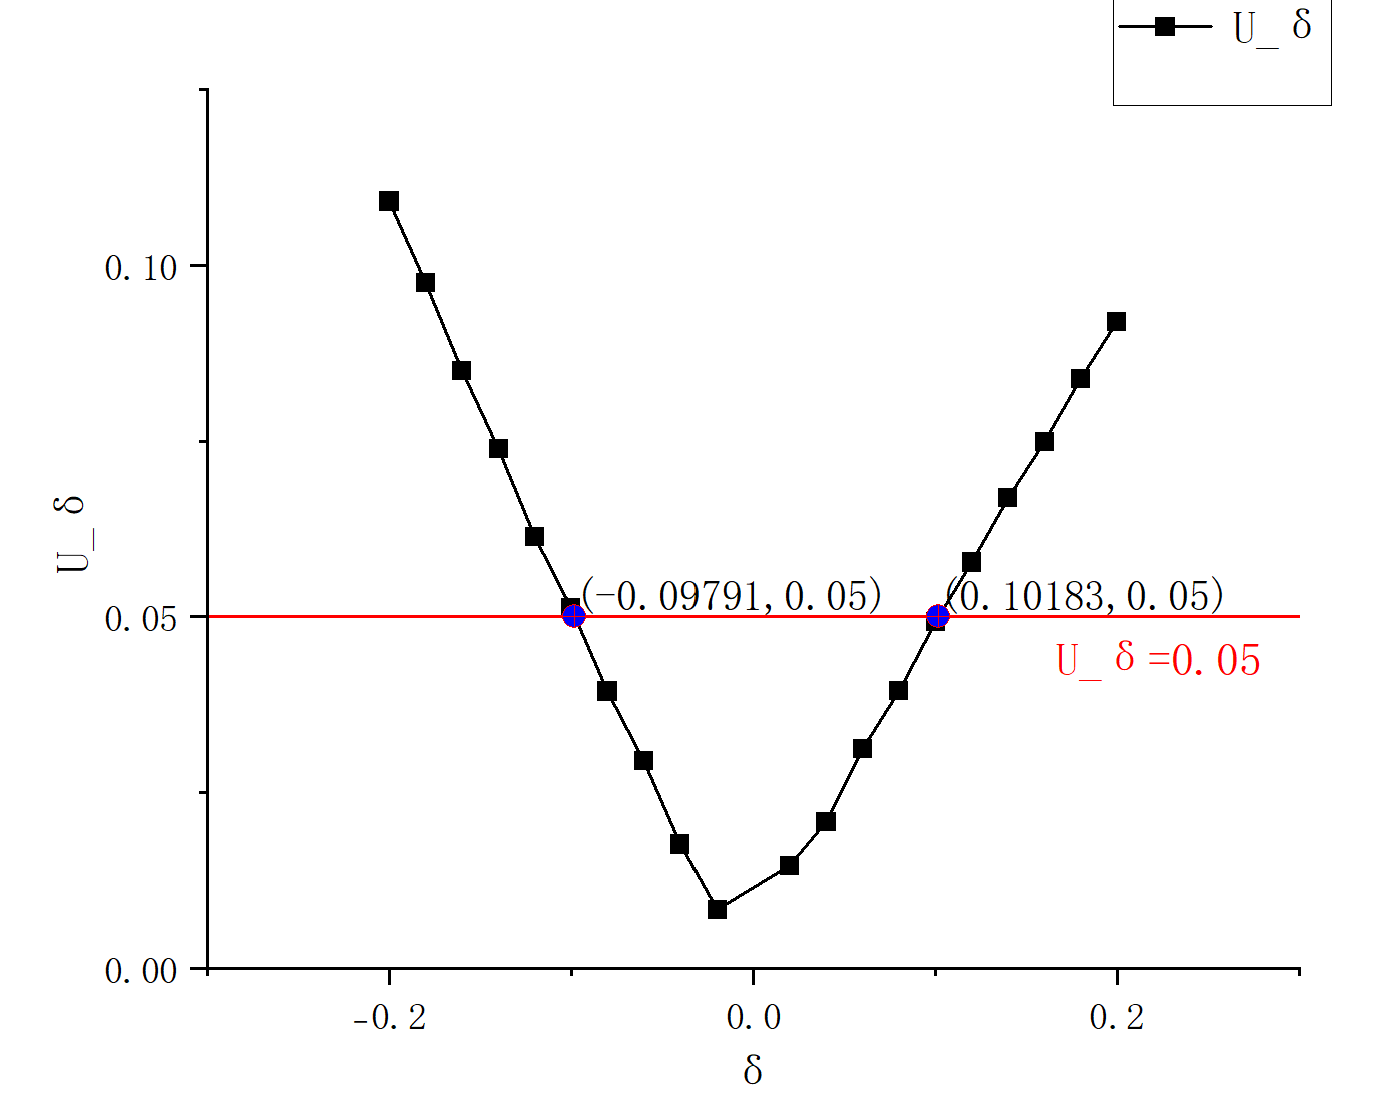
\includegraphics[scale=0.4]{3.1.2} \\\small{图4.3.2 $R_0=50\Omega$时$U_\delta -\delta $关系图}
    \end{minipage}
    ~\\

    如图4.3.1,图3.3.2所示,$U_g - \delta$线性关系成立的$\delta$取值范围为$-0.09791<\delta<0.10183$,与理论值:$-0.09524<\delta<0.10526$左误差为2.80\%,右端点误差为3.26\%,均小于5\%,误差在合理范围内。此时$R_4$取值范围为$45.1045\Omega<R_4<55.0915\Omega$。

    ~\\
    \begin{minipage}[c]{1\textwidth}
        \centering 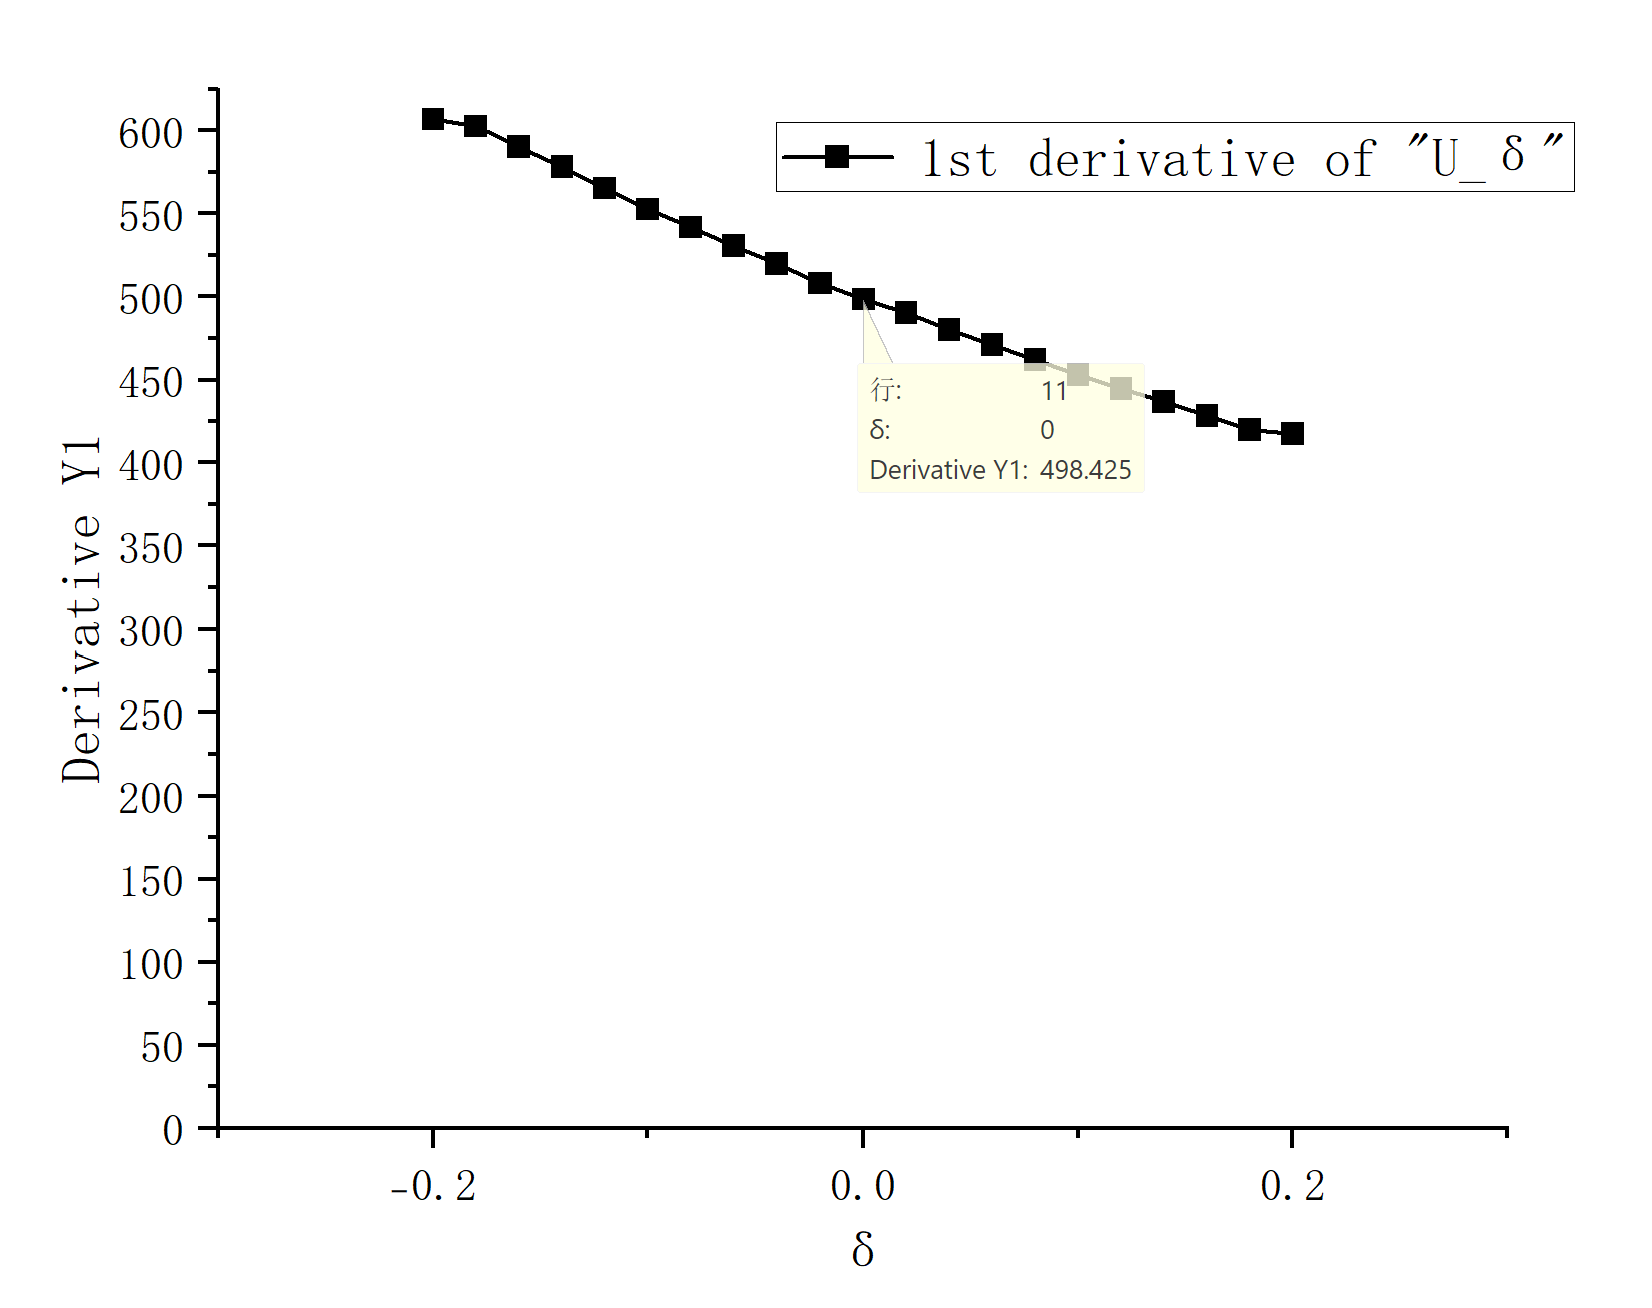
\includegraphics[scale=0.4]{3.1.3} \\\small{图4.3.3 $R_0=50\Omega$时$U_g^{\text{实际}} - \delta$拟合曲线的导数曲线}
    \end{minipage}
    ~\\

    同实验一方法,如图4.3.3所示,在$\delta=0$处,绝对灵敏度为9.9685$mV/\Omega$

    \subsubsection*{4.2.3 总结}
    综合在$R_0=1000\Omega$,$R_0=5000\Omega$,$R_0=50\Omega$下的三组数据,发现$R_0$越大,$U_g - \delta$线性关系成立的$\delta$取值范围越大,零点绝对灵敏度越小。

    \subsection*{4.3 \quad 实验三:使用非平衡电桥测量铜丝的电阻温度系数}
    测量结果如下表所示。由$R=4\dfrac{U_g-U_{gmin}}{U_S}$。
    有$U_{gmin}=0.062mV$(此电阻箱分度值下的最小值)。
    \begin{table}[!ht]
        \centering 表4:不同温度下对应的铜丝电阻
        \resizebox*{\textwidth}{!}{
            \begin{tabular}{|c|c|c|c|c|c|c|c|c|c|c|c|c|c|}
                \hline
                $T/^\circ C$       & 27.8   & 30     & 35     & 40     & 45     & 50     & 55     & 60     & 65     & 70     & 75     & 80     & 85     \\ \hline
                $U_g/mV$   & 2.179  & 2.198  & 2.233  & 2.267  & 2.298  & 2.34   & 2.379  & 2.425  & 2.466  & 2.509  & 2.545  & 2.583  & 2.62   \\ \hline
                $R/\Omega$ & 0.2117 & 0.2136 & 0.2171 & 0.2205 & 0.2236 & 0.2278 & 0.2317 & 0.2363 & 0.2404 & 0.2447 & 0.2483 & 0.2521 & 0.2558 \\ \hline
                \end{tabular}
        }
        \end{table}
        
        ~\\
        \begin{minipage}[c]{1\textwidth}
            \centering 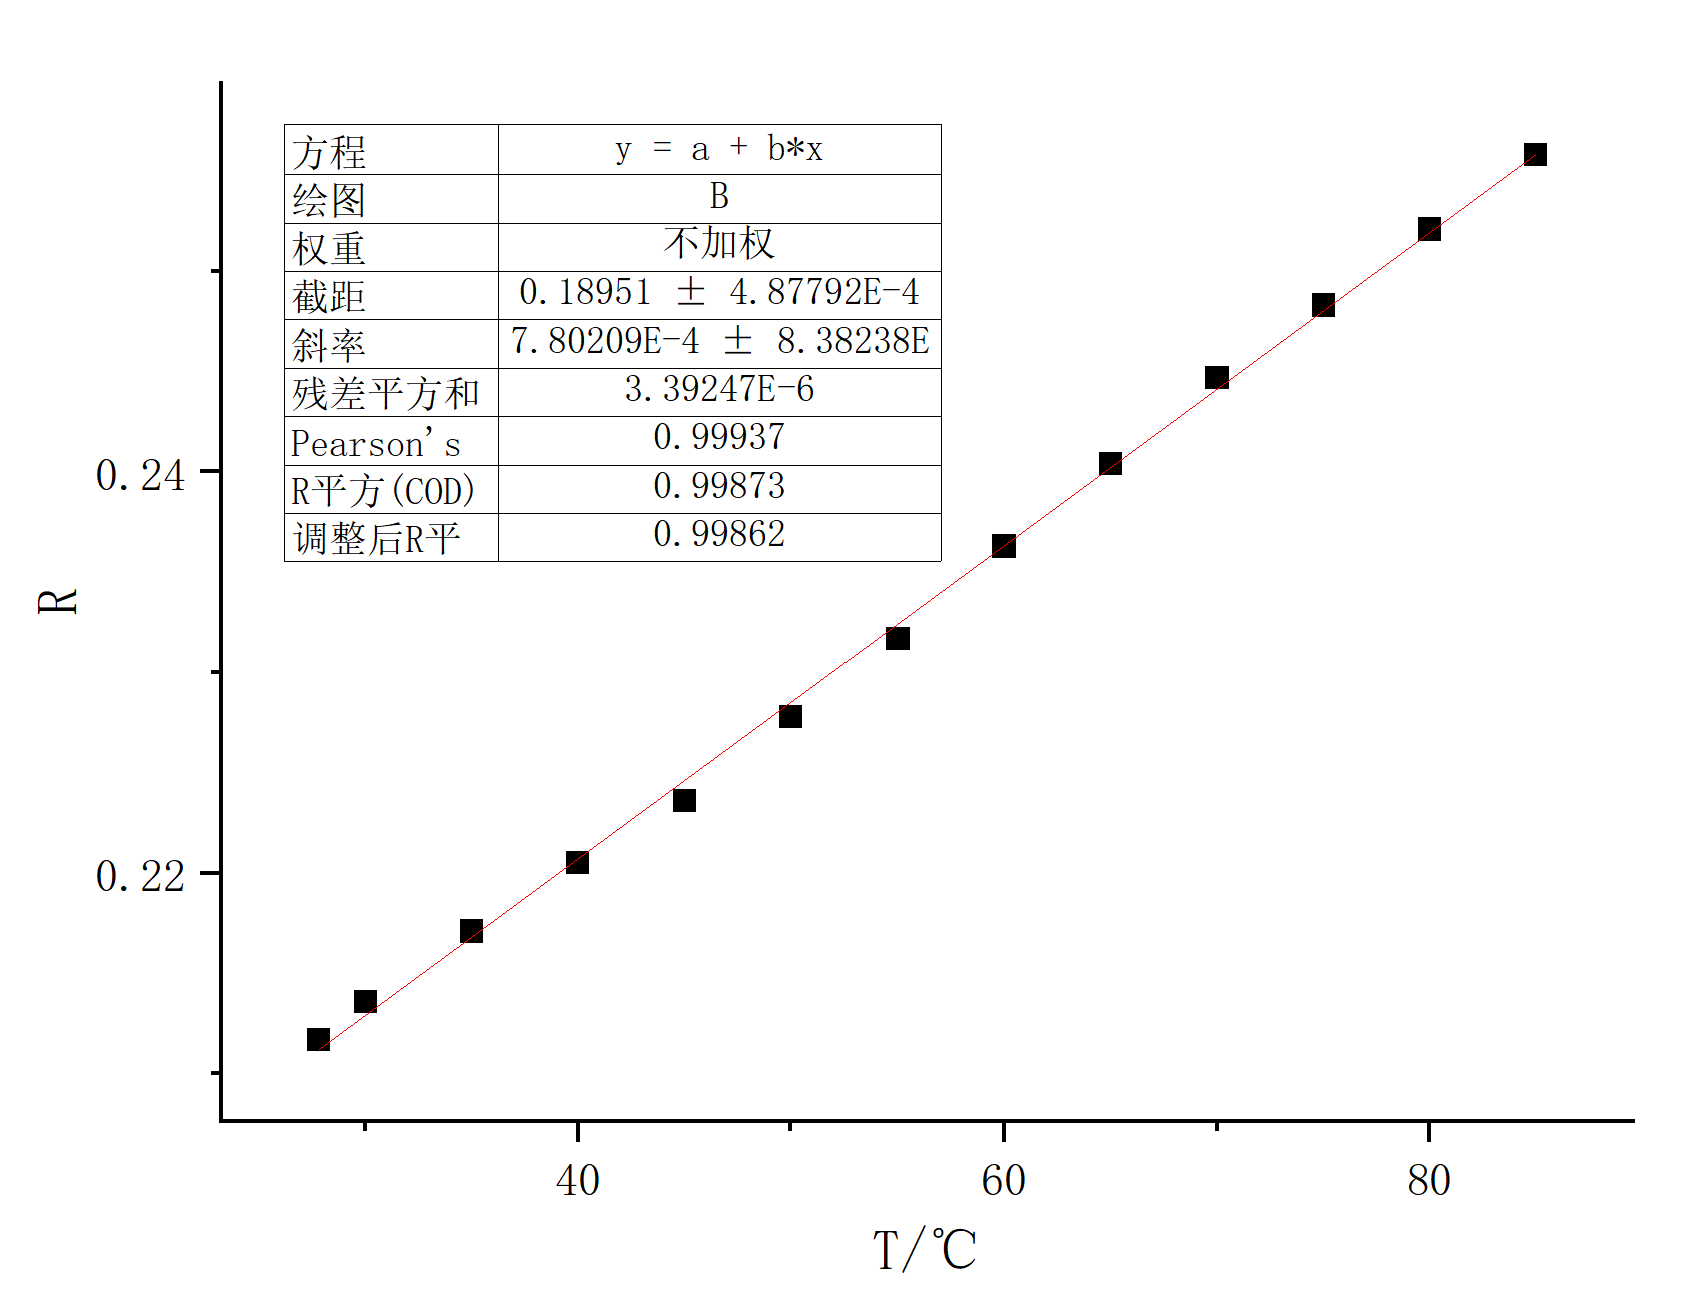
\includegraphics[scale=0.4]{5} \\\small{图5 温度与铜丝电阻的关系}
        \end{minipage}
        ~\\

        如图5所示,$R_{Cu}=7.802\times 10^{-4}t+0.1895$。由此计算出在0$^\circ C$和20$^\circ C$时铜丝电阻的拟合值分别为0.1895$\Omega$和0.2051$\Omega$。根据电阻温度系数定义公式$\alpha_T=\dfrac{k}{R_T}$,铜丝在0$^\circ C$和20$^\circ C$时电阻温度系数为0.00412$(^\circ C)^{-1}$和0.00380$(^\circ C)^{-1}$。
        
        由图5,相关系数$r=0.99937$

        斜率k的标准不确定度$u_k=k\sqrt{\dfrac{1/r^2-1}{13-2}}=8.354\times 10^{-6}$
        
        截距b的标准不确定度$u_b=\sqrt{\overline{x^2} }u_k=4.861\times 10^{-4}$

        设斜率与截距的相关系数为0,则

        相对不确定度$\dfrac{u_{\alpha}}{\alpha}=\sqrt{(\dfrac{u_k}{k})^2+(\dfrac{u_b}{b})^2}=0.011$。

        20$^\circ C$时绝对不确定度$u_{\alpha_{20}}=4.18\times 10^{-5}$。

        根据铜丝参数$\rho=0.0175\Omega\times\dfrac{mm^2}{m};l=3m;\Phi=0.60mm$,得出20$^\circ C$下,铜丝电阻为0.1857$\Omega$。与实验结果的误差达到了10.4\%。猜测可能是因为铜丝漆包线破损导致漏电使得电阻变大。


        
        \section*{第五部分\quad 思考题}
        \subsection*{6.1 简述直流非平衡电桥与直流平衡电桥的关系}
        直流平衡电桥是把待测电阻与标准电阻进行比较,通过调节电桥平衡,从而测得待测电阻值。 非平衡电桥的基本原理是通过桥式电路来测量电阻,根据电桥输出的不平衡电压,再进行简单的线性运算处理,从而得到电阻的变化量。

        因此,直流非平衡电桥可以看作是直流平衡电桥的一种扩展应用形式,用于测量无法通过平衡条件精确测量的连续变化的物理量。

        \subsection*{6.2 为什么在实验内容 1 中, $\Delta R_4$的绝对值相同时,$R_4$小于 $1000\Omega$ 时的$U_g$值比$R_4$大于$1000\Omega$时的$U_g$值, 绝对值大?}
        由(2)式
        $$U_g=\dfrac{U_s}{4} \delta \dfrac{1}{1+\frac{1}{2}\delta}\quad (2)$$

        求导得

        $$U_g^\text{'}=\dfrac{U_s}{4}\dfrac{4}{(2+\delta)^2}$$

        故当$\delta<0$时的$U_{g}^\text{'}$大于$\delta>0$时的$U_{g}^\text{'}$,$R_4$小于 $1000\Omega$ 时的$U_g$变化率更大,故在$\Delta R_4$的绝对值相同时,$U_g$的绝对值更大。此点在图4.1.3,图4.2.3,图4.3.3中也有体现。

        \subsection*{6.3 假设用非平衡电桥来测量一个热敏电阻的电阻值随温度的变化, $U_s$= 2.0V,毫伏表
        最小刻度为 1 mV,在室温(35$^\circ C$) 到 85$^\circ C$度范围内,热敏电阻的电阻值改变 50 Ω。
        取等臂电桥,为了保证测量的灵敏度(即:每隔 5$^\circ C$读一次输出电压值,变化量不
        小于 1mV) 并且保持(与理论线性之间的)误差小于 5\%的线性范围,请问$R_0$取多
        少比较合适? (指取值范围的上、 下限。)}

        $\delta=\dfrac{\Delta R}{R_0}$的理论范围为$-\dfrac{10}{105}<\delta<\dfrac{10}{95}$,本实验中要求量程为50$\Omega$,初始处于零点位置,同时并不确定热敏电阻是正温度系数还是负温度系数,因此取$\delta$小值进行计算。代入$\Delta R=50\Omega$得到$R_0=525\Omega$。故下限为$R_0=525\Omega$。

        理论上电桥在零点附近的绝对灵敏度$S=\lim_{\Delta R \to 0}\dfrac{\Delta U_g}{\Delta R}=\dfrac{U_s}{4R_0}  $
        本实验中要求电阻改变5$\Omega$电压改变不小于1mV,即在零点附近的绝对灵敏度不小于0.2$mV/\Omega$,即为$R_0<2500\Omega$。

        故$525\Omega<R_0<2500\Omega$。

        \subsection*{6.4 把计算出来的 Cu 丝电阻温度系数(t=20℃) 与参考值 0.00393$(^\circ C)^{−1}$进行比较, 并
        分析测量的精确程度,以及产生误差的可能原因。}
        测量值为0.00380$(^\circ C)^{-1}$,误差为3.3\%。由于实验中测量温度方法较为粗糙,可能存在测量温度不准确;同时不同的Cu丝可能有微小的差异,导致温度系数不同。因此该误差可以认为在合理范围内。

        \section*{第六部分\quad 结论}
        通过本次实验,我们得知了非平衡电桥的线性区间和灵敏度受到桥臂电阻$R_0$的影响,$R_0$越大,$U_g - \delta$线性关系成立的$\delta$取值范围越大,即非平衡电桥的量程越大,但同时零点绝对灵敏度越小,测量精度下降。
        
        非平衡电桥具有精度高、响应速度快、适用范围广等优点,通过使用非平衡电桥,可以精密测量电阻。除了用来测量铜丝的电阻温度系数,在工程中,非平衡电桥还被广泛应用于传感器、仪器仪表、自动控制系统等领域,为各行各业的产品和系统提供了更精准的测量手段,有助于提高工业生产效率和产品质量。

    \section*{致谢}
\begin{center}
	感谢中国科学技术大学物理实验教学中心和郭玉刚老师
\end{center}
\label{unknown}
\end{document}